%--------------------------------------------------------------------------------------%
%
%	The file 'patent.tex' is a file with the intent of being using for patent application drafts.
%   This is a revamped version from the original document created by Nettimi (see source #1),
%   and with the information presented in the European Patent Office (EPO) patent application
%   draft example for european patents
%      
% 
% 	Author: Saúl S. Carvalho
%
%
%
%   This work may be distributed and/or modified under the conditions 
%   of the TeXstudio Public License, either version 4.3.1 of 
%   this license or (at your option) any later version.  
%   The latest version of the license is available at 
%   https://www.texstudio.org/license.txt.  
%   Version 4.3.1 or later is included with all distributions 
%   of TeXstudio version 4.3.1 or later.
%
%   Content Source #1: Indian-Patent-Drawings-LaTeX-Template repository by Nettimi Srinivas
%   Content Source #2: Patent Application Draft Example from European Patent Office (EPO)
% 
%
%--------------------------------------------------------------------------------------%

\documentclass[10pt, a4paper]{article}

%------------------------%
% Include LaTeX packages %
%------------------------%

\usepackage[top=3cm, left=3cm, bottom=3cm, right=3cm]{geometry}
\usepackage{graphicx}
\usepackage{rotating}
\usepackage{subfigure}

\usepackage{amsmath,amssymb,amsfonts}
\usepackage{algorithmic}

\usepackage{mathtools}

\usepackage{ifpdf}
\usepackage{float}
\usepackage{pdfpages}
\usepackage{epstopdf}
\usepackage{array}

\usepackage{tabulary}
\usepackage{multirow}
\usepackage{enumitem}
\usepackage{textcomp}
\usepackage{ragged2e}
\usepackage{soul}
\usepackage{arydshln}
\usepackage[normalem]{ulem}

\usepackage[numbers,sort&compress]{natbib}
\usepackage{booktabs}
\usepackage{cite}

\usepackage{caption}
\captionsetup[figure]{name={FIG.}, labelsep=space, justification=centering, singlelinecheck=false}
\usepackage{subcaption}

\usepackage{lastpage}

\usepackage{fancyhdr}	
\pagestyle{fancy}
\renewcommand{\headrulewidth}{0.0pt}
\setlength{\parindent}{0pt}
\setlength\headheight{30pt}

% New commands for the writing of the patent
\newcommand{\mypatenttitle}[1]{\textbf{\underline{#1}}\\}
\newcommand{\mytitle}[1]{#1\\}
\newcommand{\myabstract}[1]{
	\begin{center}
		ABSTRACT
	\end{center}	
	\normalsize
	#1
}
\newcommand{\mydescription}[1]{
	\begin{center}
		DESCRIPTION
	\end{center}	
	\normalsize
	#1
}
\newcommand{\mydescriptionline}[2]{
	\textbf{#1}\\\\
	\normalsize
	#2\\\\
}
\newcommand{\myfiguredescription}[2]{%
	\normalsize
	Fig. #1 is #2.\\
}
\newcommand{\myclaims}[1]{
	\begin{center}
		CLAIMS
	\end{center}	
	\normalsize
	#1
}
\newcommand{\myclaimsline}[3]{
	\normalsize
	#1. #2\\\\
}
\newcommand{\mydrawings}[1]{
	\begin{center}
		DRAWINGS
	\end{center}	
	#1
}



%-----------------------%
% Headers and Footnotes %
%-----------------------%

	\lhead
	{
		Applicant: 
	    { % Enter the applicant(s) name(s) here
	    	Enter Applicant(s) Name  		
    	}\\
		Patent Application Number:
		{ % Enter your application number here
			Enter App. no.
		}
	}
    
	\rhead
	{	
		Total No. of Sheets: \pageref{LastPage}\\
		Sheet No.: \thepage
  	}
  
	\rfoot{}
	
	\cfoot{}
	
	
	
%---------------------%
% Document  Beginning %
%---------------------%	
	
\begin{document}
	\myabstract{
		% Here you put your patent title
		\mypatenttitle{Pedalling device for bicycle}
		
		% Here you put your patent's abstract text
		A pedalling device for a bicycle includes a support seat (13), a rotation shaft (111), a chainwheel (11), two opposite oneway ratchet wheels (40), two opposite drive members (30), a crank (12), two opposite drive shafts (141), two pedals (14), and two opposite slide seats (50). Thus, the drive members have a longer force arm between the crank and the chainwheel so as to increase the force moment of the pedalling device so that the rider can step the pedals in an energy-saving manner, thereby saving the rider's energy and manual work.
	}
	
	% Here you start describing your patent
	\mydescription{
		% Description line #1
		\mydescriptionline{Pedalling device for bicycle}{ }	
		% Description line #2
		\mydescriptionline{Technical field to which invention relates}{
			The present invention relates to a pedalling device and, more particularly, to a pedalling
			device for a bicycle.
		}	\\
		% Description line #3
		\mydescriptionline{Indication of background art}{
			A conventional pedalling device for a bicycle in accordance with the prior art shown in Fig. 10 comprises a crank 60, two pedals 61, a chainwheel 62, and a chain 64. Thus, when the	crank 60 is driven by the pedals 61, the chainwheel 62 is rotated by the crank 60 to drive the chain 64 so as to move the bicycle. However, the force arm defined between the center of the chainwheel 62 and each of the pedals 61 has a smaller length, so that the rider has to exert a larger stepping force on the pedals 61 so as to move the bicycle, thereby greatly wasting the rider's energy and manual work. 
		}	\\
		% Description line #4
		\mydescriptionline{Technical problem to be solved}{
			The objective of the present invention is to provide a pedalling device, and more particular a pedalling device for a bicycle, wherein the rider can step the pedals in an energy-saving manner. 
		}	\\
		% Description line #5
		\mydescriptionline{Disclosure of invention}{
			In accordance with the present invention, there is provided a pedalling device, comprising
			a support seat, a rotation shaft rotatably mounted on a first end of the support seat, a
			chainwheel secured on and rotated by the rotation shaft, two opposite oneway ratchet
			wheels each mounted on the rotation shaft to rotate the rotation shaft, two opposite drive
			members each having a first end formed with a ratchet socket mounted on a respective
			ratchet wheel to rotate the respective ratchet wheel in a oneway manner and a second end
			formed with on elongate slide track, a crank pivotally mounted on a second end of the
			support seat, two opposite drive shafts secured on two opposite sides of the crank to
			rotate the crank, two pedals each rotatably mounted on a respective drive shaft, and two
			opposite slide seats each pivotally mounted on a respective drive shaft to move therewith
			and each slidably mounted in the slide track of a respective drive member. \newline
			
			Advantageously, the drive members have a longer force arm between the crank and the chainwheel so as to increase the force moment of the pedalling device, thereby saving the rider’s energy and manual work. \newline
			
			Further benefits and advantages of the present invention will become apparent after a careful reading of the detailed description with appropriate reference to the accompanying drawings. 
		}	\\
		% Description line #6
		\mydescriptionline{Brief description of drawings}{
			\myfiguredescription{1}{a perspective view of a pedalling device in accordance with the preferred embodiment of the present invention}
			\myfiguredescription{2}{an exploded perspective view of the pedalling device as shown in Fig. 1}
			\myfiguredescription{3}{a plan view of the pedalling device for a bicycle as shown in Fig. 1}
			\myfiguredescription{4}{a plan cross-sectional view of the pedalling device as shown in Fig. 1}
			\myfiguredescription{5}{a plan cross-sectional view of the pedalling device as shown in Fig. 1}
			\myfiguredescription{6}{a plan cross-sectional operational view of the pedalling device as shown in Fig. 1}
			\myfiguredescription{7}{a locally enlarged view of the pedalling device as shown in Fig. 6}
			\myfiguredescription{8}{a schematic operational view of the pedalling device as shown in Fig. 6}
			\myfiguredescription{9}{a schematic operational view of the pedalling device as shown in Fig. 7}
			\myfiguredescription{10}{is a perspective view of a conventional pedalling device for a bicycle in accordance with the prior art}	
		} \\
		% Description line #7
		\mydescriptionline{Description of at least one way of carrying out the invention}{
			Referring to the drawings and initially to Figs. 1-7, a pedalling device 20 for a bicycle 10 in accordance with the preferred embodiment of the present invention comprises a support
			seat 13, a rotation shaft 111 rotatably mounted on a first end of the support seat 13, a
			chainwheel 11 secured on and rotated by the rotation shaft 111, two opposite oneway
			ratchet wheels 40 each mounted on the rotation shaft 111 to rotate the rotation shaft 111,
			two opposite drive members 30 each having a first end formed with a ratchet socket 31
			mounted on a respective ratchet wheel 40 to rotate the respective ratchet wheel 40 in a
			oneway manner and a second end formed with an elongate slide track 35, a crank 12
			pivotally mounted on a second end of the support seat 13, two opposite drive shafts 141
			secured on two opposite sides of the crank 12 to rotate the crank 12, two pedals 14 each
			rotatably mounted on a respective drive shaft 141, and two opposite slide seats 50 each
			pivotally mounted on a respective drive shaft 141 to move therewith and each slidably
			mounted in the slide track 35 of a respective drive member 30.
			The rotation shaft 111 has two opposite ends each formed with 5 hexagonal fixing stud
			112 and a threaded rod 113. \newline
			
			Each of the ratchet wheels 40 includes an inner part 45 formed with a hexagonal fixing
			hole 42 secured on the fixing stud 112 of the rotation shaft 111 to rotate the rotation shaft 111, an outer part 43 rotatably mounted on the inner part 45 and having an outer wall
			formed with a driven gear 41 and an inner wall formed with a plurality of locking grooves
			430,and a plurality of oneway detents 44 each having a first end pivotally mounted on the
			inner part 45 and a second end engaged in the respective locking groove 430 of the outer
			part 43. \newline
			
			The ratchet socket 31 of each of the drive members 30 has an inner wall formed with a
			drive gear 311 meshing with the driven gear 41 of the respective ratchet wheel 40 to rotate
			the respective ratchet wheel 40. The ratchet socket 31 of each of the drive members 30 is
			combined with the respective ratchet wheel 40 by two opposite seal rings 32 which are
			located at two opposite sides of the ratchet socket 31 of each of the drive members 30 and
			are fastened by a plurality of rivets 33. \newline
			
			The pedalling device 20 further comprises two washers 37 each mounted on a respective
			threaded rod 113 of the rotation shaft 111 and each rested on a respective ratchet wheel 40, and two nuts 34 each screwed onto a respective threaded rod 113 of the rotation shaft
			111 and each rested on a respective washer 37. \newline
			
			The second end of the support seat 13 is formed with a pivot hole 131. The crank 12 is
			pivotally mounted in the pivot hole 131 of the support seat 13. Each of the two sides of the crank 12 has a distal end formed with a screw bore 121. Each of the two drive shafts 141 has a threaded distal end screwed into the respective screw bore 121 of the crank 12 to
			secure each of the drive shafts 141 to the crank 12. \newline
			
			Each of the two slide seats 50 has a first end provided with two first bearings 51 slidably
			mounted in the slide track 35 of the respective drive member 30 and a second end
			provided with a sleeve 52 for mounting two second bearings 53 which are pivotally
			mounted on the respective drive shaft 141. The first bearings 51 of each of the two slide
			seats 50 are limited in the slide track 35 of the respective drive member 30 by an end cap
			36 which is mounted on an opened end of the slide track 35 to prevent the first bearings
			51 of each of the two slide seats 50 from being detached from the slide track 35 of the
			respective drive member 30. \newline
			
			In operation, referring to Figs. 1-9, when the pedals 14 are stepped by the rider, the crank 12 is rotated to move the two slide seats 50 which are moved upward and downward to
			drive the drive members 30 to pivot upward and downward as shown in Fig. 6, so that the
			ratchet socket 31 of each of the drive members 30 is rotated to rotate the respective
			ratchet wheel 40. \newline
			
			As shown in Fig. 7, when one of the drive members 30 is pivoted downward, the
			respective ratchet wheel 40 is rotated clockwise to rotate the outer part 43. At this time, the oneway detents 44 of each of the ratchet wheels 40 are engaged in the locking grooves 430 of the outer part 43, so that the inner part 45 is driven and rotated by the outer part 43 to rotate the fixing hole 42 which rotates the fixing stud 112 of the rotation shaft 111 so as to rotate the rotation shaft 111. Thus, when the ratchet wheel 40 is rotated clockwise, the rotation shaft 111 is rotated to rotate the chainwheel 11 so as to move the bicycle. On the contrary, when one of the drive members 30 is pivoted upward as shown in Fig. 8, the respective ratchet wheel 40 is rotated counterclockwise to rotate the outer part 43 as shown in Fig. 9. At this time, the oneway detents 44 of each of the ratchet wheels 40 are disengaged from the locking grooves 430 of the outer part 43, so that the inner part 45 is not rotated by the outer part 43, and the outer part 43 performs an idle rotation. Thus, when the ratchet wheel 40 is rotated counterclockwise, the rotation shaft 111 stops rotating, so that the chainwheel 11 stops rotating. \newline
			
			In such a manner, when one of the drive members 30 is pivoted upward as shown in Fig.
			8, the other one of the drive members 30 is pivoted downward as shown in Fig. 6, so that
			the chainwheel 11 is rotated successively so as to move the bicycle successively. \newline
			
			Accordingly, the drive members 30 have a longer force arm between the crank 12 and the
			chainwheel 11 so as to increase the force moment of the pedalling device 20 so that the
			rider can step the pedals 14 in an energy-saving manner, thereby saving the rider’s energy
			and manual work. \newline
			
			Although the invention has been explained in relation to its preferred embodiment(s) as
			mentioned above, it is to be understood that many other possible modifications and
			variations can be made without departing from the scope of the present invention. It is,
			therefore, contemplated that the appended claim or claims will cover such modifications
			and variations that fall within the true scope of the invention. 
		} \\
	}
	
	% Here you add your patent's claims
	\myclaims{
		\myclaimsline{1}{A pedalling device, comprising: \\
			a support seat (13); \\
			a rotation shaft (111) rotatably mounted on a first end of the support seat (13);  \\
			a chainwheel (11) secured on and rotated by the rotation shaft (111); \\
			two opposite oneway ratchet wheels (40) each mounted on the rotation shaft (111) to
			rotate the rotation shaft (111); \\
			two opposite drive members (30) each having a first end formed with a ratchet socket (31)
			mounted on a respective ratchet wheel (40) to rotate the respective ratchet wheel (40) in a
			oneway manner and a second end formed with an elongate slide track (35); \\
			a crank (12) pivotally mounted on a second end of the support seat (13); \\
			two opposite drive shafts (141) secured on two opposite sides of the crank (12) to rotate
			the crank (12); \\
			two pedals (14) each rotatably mounted on a respective driveshaft (141); \\
			two opposite slide seats (50) each pivotally mounted on a respective drive shaft (141) to
			move therewith and each slidably mounted in the slide track (35) of a respective drive
			member (30).
		} \\
		\myclaimsline{2}{The pedalling device in accordance with claim 1, wherein: \\
			the rotation shaft (111) has two opposite ends each formed with hexagonal fixing stud
			(112) and a threaded rod (113); \\
			each of the ratchet wheels (40) includes an inner part (45) formed with a hexagonal fixing
			hole (42) secured on the fixing stud (112) of the rotation shaft (111) to rotate the rotation shaft (111), and an outer part (43) rotatably mounted on the inner part (45) and having an outer wall formed with a driven gear (41); \\
			the ratchet socket (31) of each of the drive members (30) has an inner wall formed with a
			drive gear (311) meshing with the driven gear (41) of the respective ratchet wheel (40) to
			rotate the respective ratchet wheel (40). 
		} \\
		\myclaimsline{3}{The pedalling device in accordance with claim 2, further comprising two washers (37) each mounted on a respective threaded rod (113) of the rotation shaft (111) and each rested on a respective ratchet wheel (40), and two nuts (34) each screwed onto a respective threaded rod (113) of the rotation shaft (111) and each rested on a respective washer (37).  
		} \\
		\myclaimsline{4}{The pedalling device in accordance with claim 2, wherein the ratchet socket (31) of each of the drive members (30) is combined with the respective ratchet wheel (40) by two opposite seal rings (32).  
		} \\
		\myclaimsline{5}{The pedalling device in accordance with claim 4, wherein the seal rings (32) are located at two opposite sides of the ratchet socket (31) of each of the drive members (30) and are fastened by a plurality of rivets (33). 
		} \\
		\myclaimsline{6}{The pedalling device in accordance with claim 1, wherein each of the two slide seats (50) has a first end provided with two first bearings (51) slidably mounted in the slide track (35) of the respective drive member (30) and a second end provided with a sleeve (52) for mounting two second bearings (53) which are pivotally mounted on the respective drive shaft (141).
		} \\
		\myclaimsline{7}{The pedalling device in accordance with claim 6, wherein the first bearings (51) of each of the two slide seats (50) are limited in the slide track (35) of the respective drive member (30) by an end cap (36) which is mounted on an opened end of the slide track (35) to prevent the first bearings (51) of each of the two slide seats (50) from being detached from the slide track (35) of the respective drive member (30). 
		} \\
		\myclaimsline{8}{The pedalling device in accordance with claim 1, wherein the second end of the support seat (13) is formed with a pivot hole (131), and the crank (12) is pivotally mounted in the pivot hole (131) of the support seat (13). 
		} \\
		\myclaimsline{9}{The pedalling device in accordance with claim 1, wherein each of the two sides of the crank (12) has a distal end formed with a screw bore (121), and each of the two drive shafts (141) has a threaded distal end screwed into the respective screw bore (121) of the crank (12) to secure each of the drive shafts (141) to the crank (12).
		} \\
		\myclaimsline{10}{The pedalling device in accordance with claim 1, wherein the outer part of each of the ratchet wheels (40) has an inner wall formed with a plurality of locking grooves (430), and each of the ratchet wheels (40) further includes a plurality of oneway detents (44) each having a first end pivotally mounted on the inner part and a second end engaged in the respective locking groove (430) of the outer part (43). 
		} \\
	}
	
	
	\mydrawings{
		\begin{figure}[!h]
			\begin{minipage}{0.49\textwidth}
				\centering
				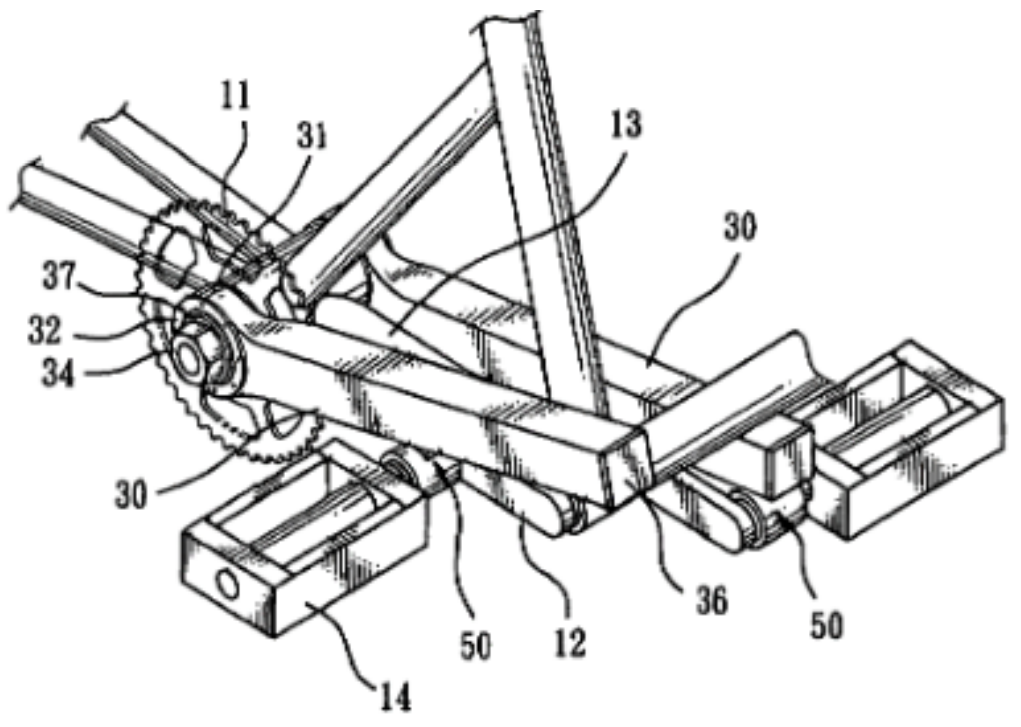
\includegraphics[width=0.8\textwidth]{figures/fig1.png}
				\caption{}
			\end{minipage}
			\begin{minipage}{0.49\textwidth}
				\centering
				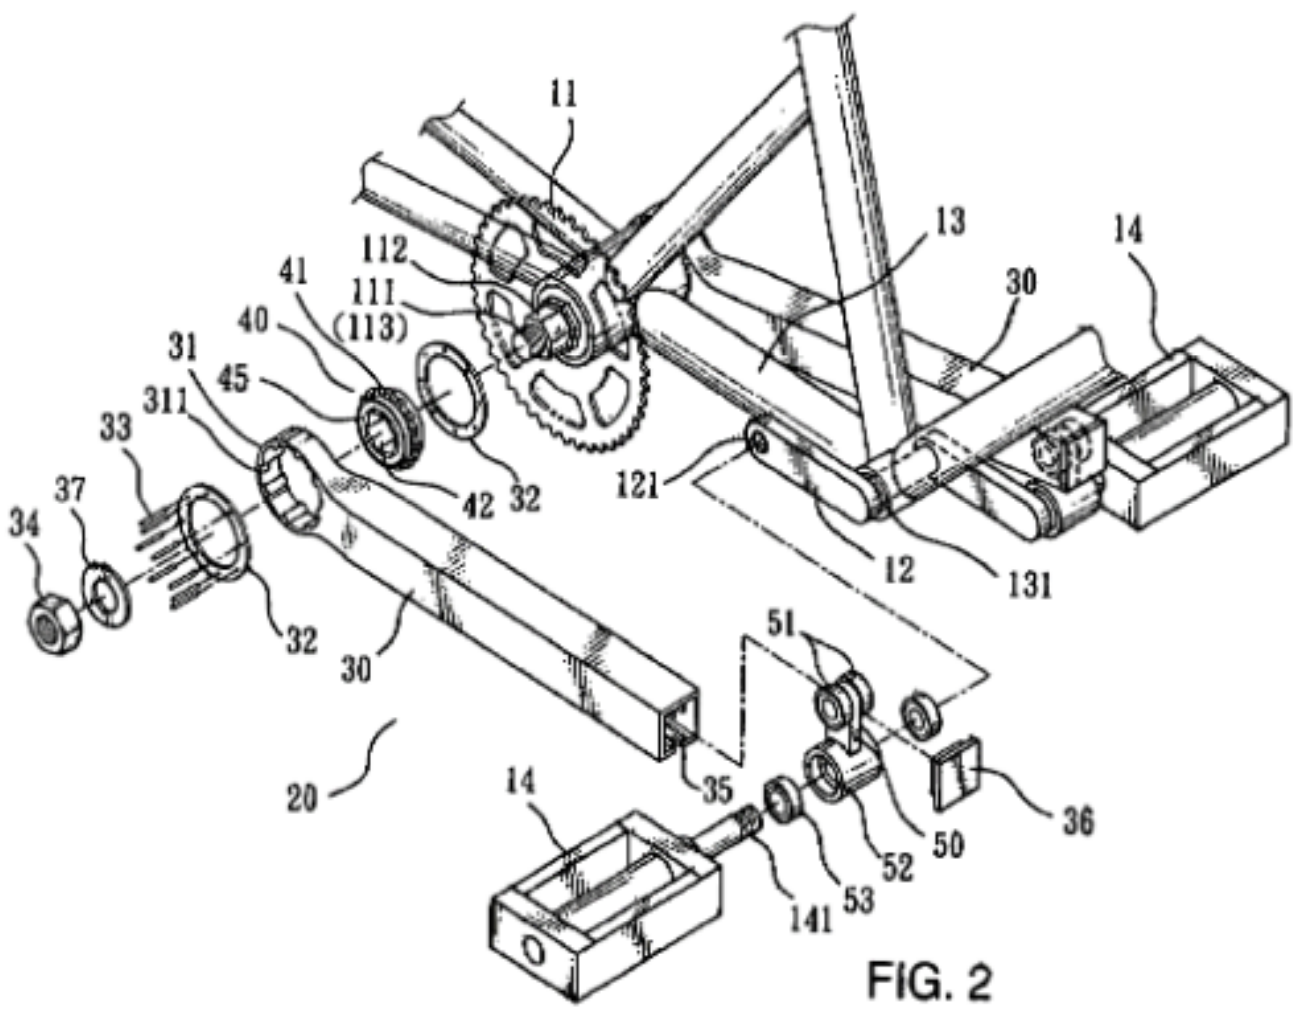
\includegraphics[width=\textwidth]{figures/fig2.png}
				\caption{}
			\end{minipage}
		\end{figure}
	
		\begin{figure}[!h]
			\begin{minipage}{0.49\textwidth}
				\centering
				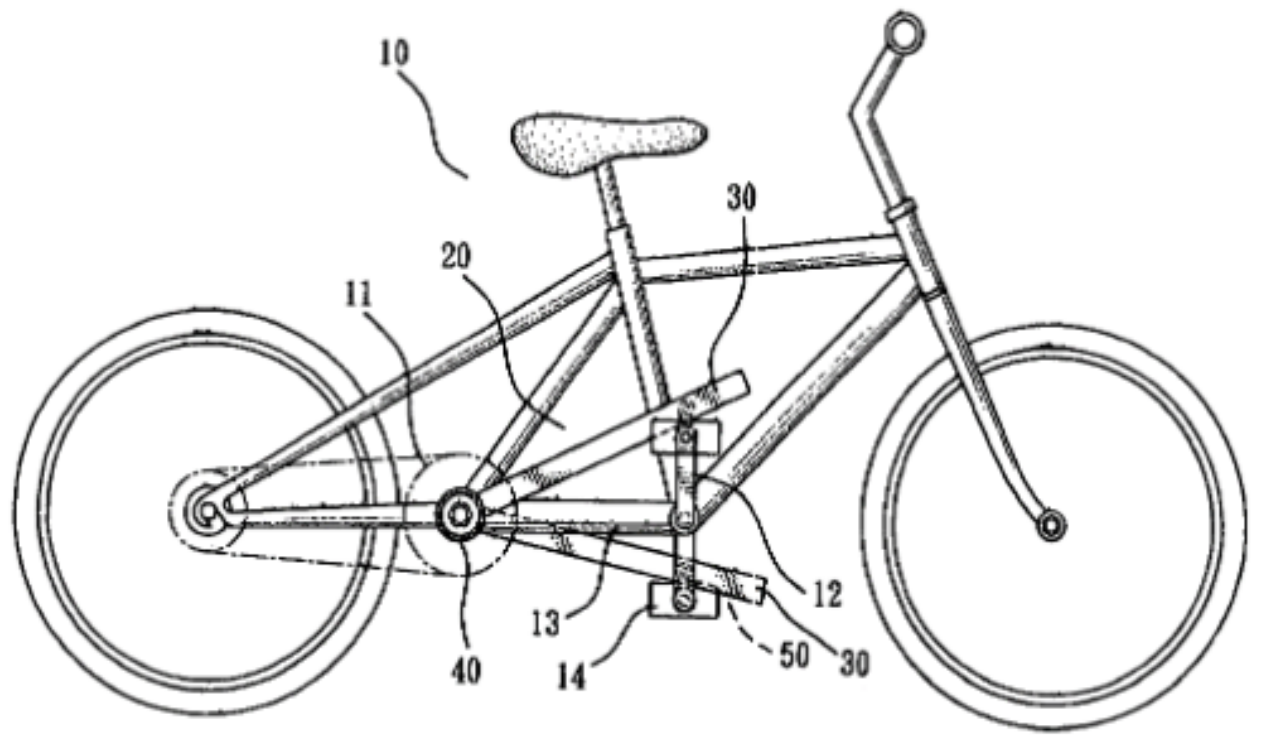
\includegraphics[width=\textwidth]{figures/fig3.png}
				\caption{}
			\end{minipage}
			\begin{minipage}{0.49\textwidth}
				\centering
				\begin{minipage}{0.49\textwidth}
					\centering
					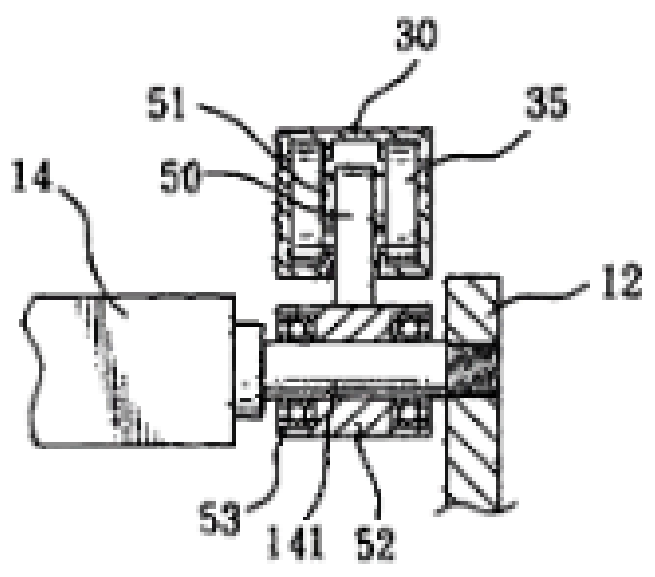
\includegraphics[width=0.8\textwidth]{figures/fig4.png}
					\caption{}
				\end{minipage}
				\begin{minipage}{0.49\textwidth}
					\centering
					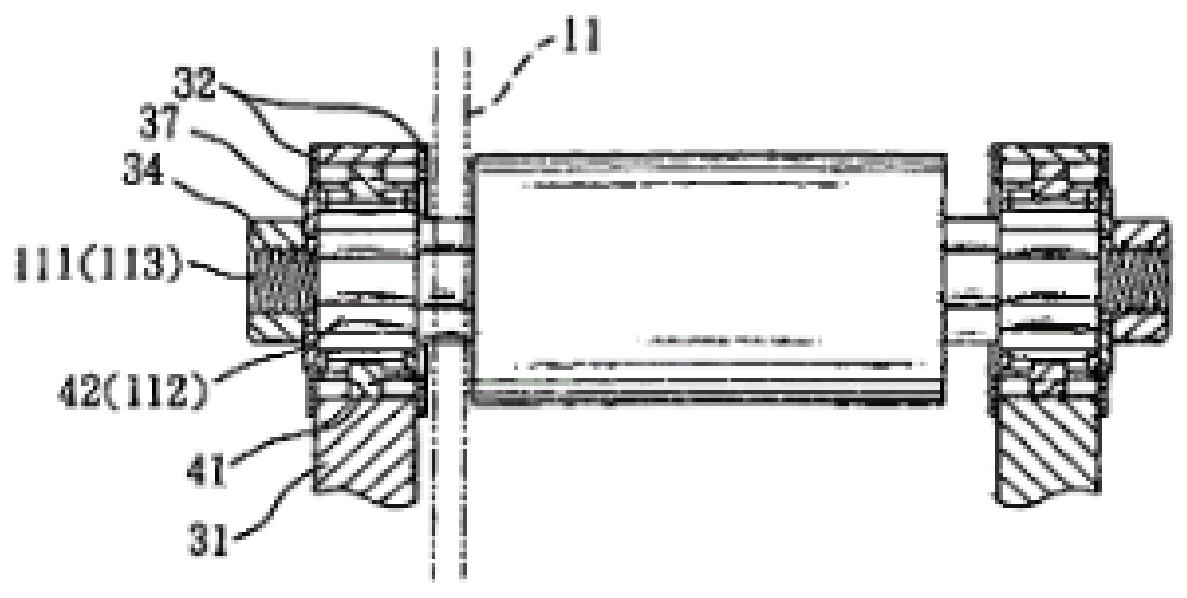
\includegraphics[width=1.1\textwidth]{figures/fig5.png}
					\caption{}
				\end{minipage}
				\begin{minipage}{0.49\textwidth}
					\centering
					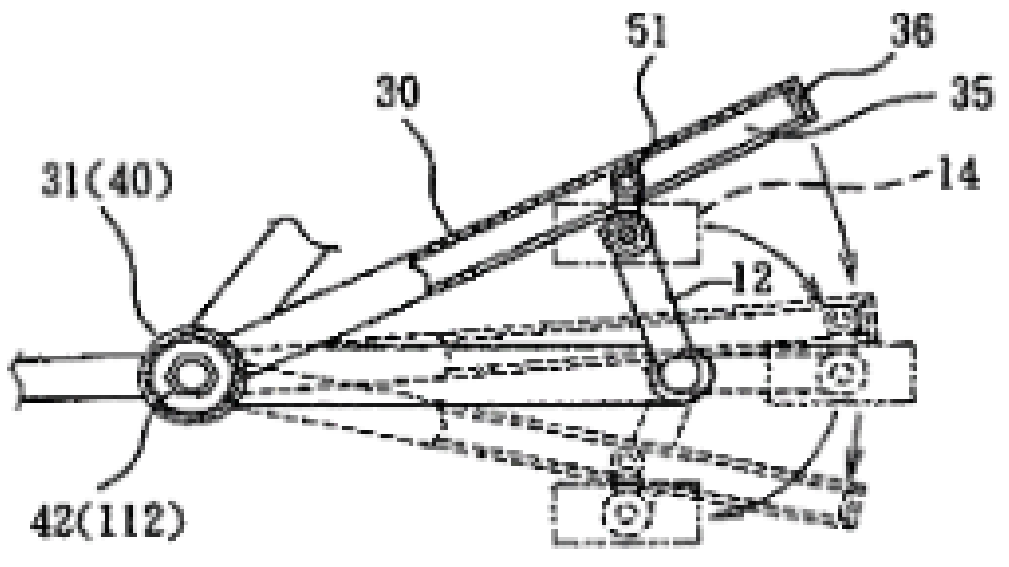
\includegraphics[width=0.9\textwidth]{figures/fig6.png}
					\caption{}
				\end{minipage}
				\begin{minipage}{0.49\textwidth}
					\centering
					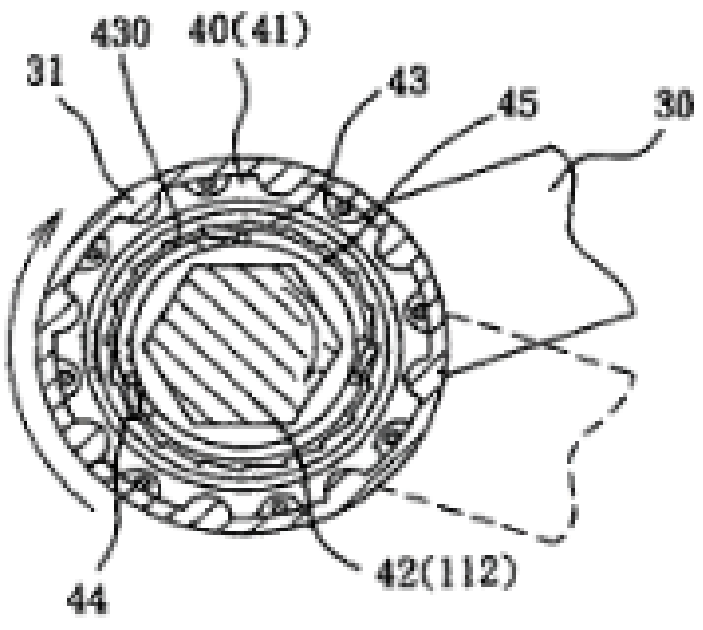
\includegraphics[width=0.8\textwidth]{figures/fig7.png}
					\caption{}
				\end{minipage}
			\end{minipage}
		\end{figure}
	
		\clearpage\newpage
		
		
		
		\begin{figure}[!h]
			\begin{minipage}{0.49\textwidth}
				\centering
				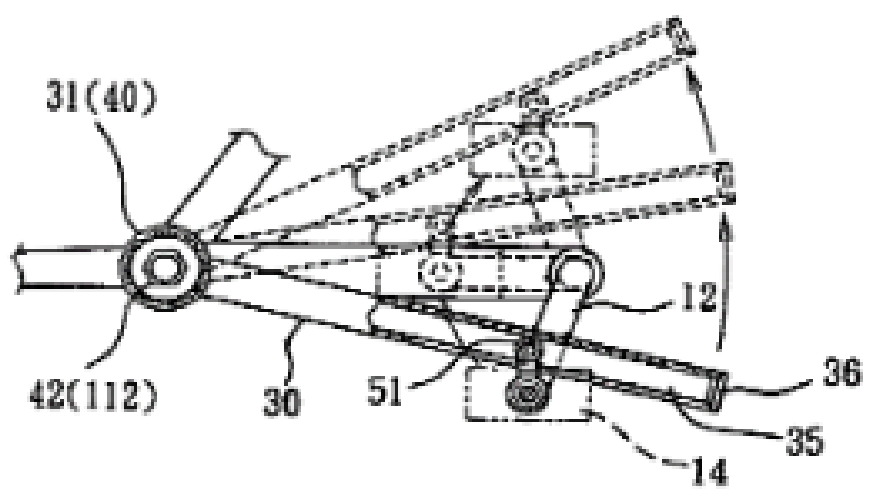
\includegraphics[width=0.8\textwidth]{figures/fig8.png}
				\caption{}
			\end{minipage}
			\begin{minipage}{0.49\textwidth}
				\centering
				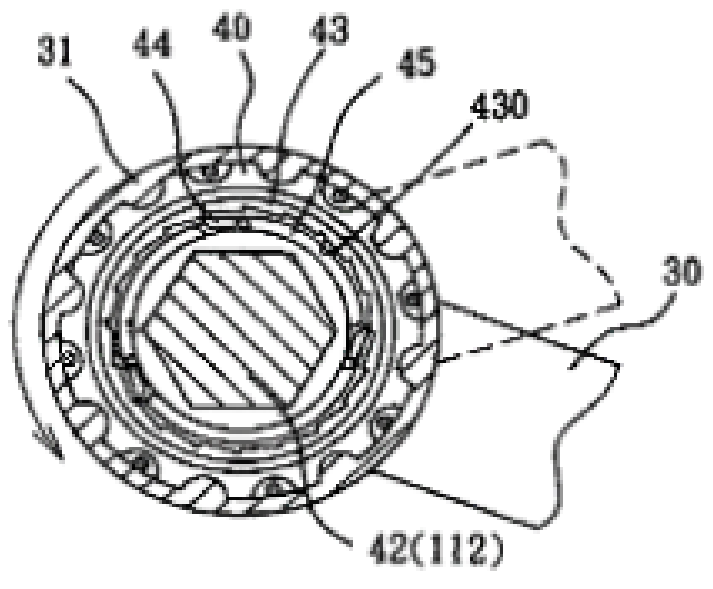
\includegraphics[width=0.8\textwidth]{figures/fig9.png}
				\caption{}
			\end{minipage}
		\end{figure}
	
		\begin{figure}[!h]
			\centering
			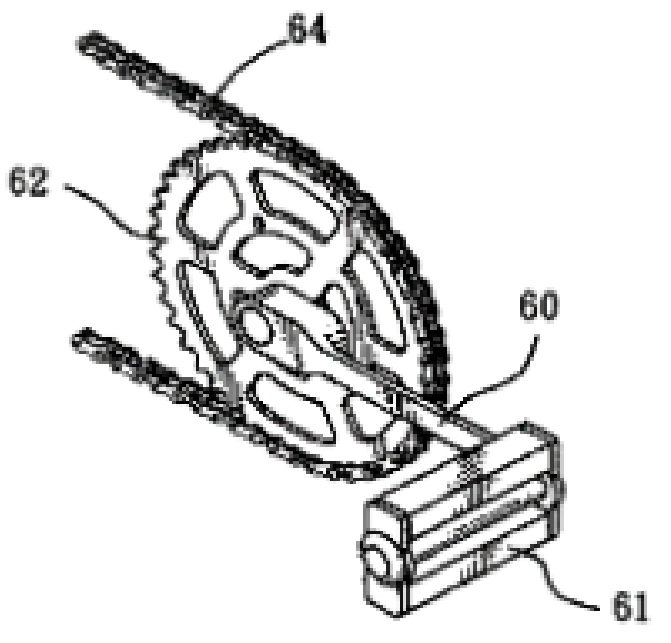
\includegraphics[width=0.4\textwidth]{figures/fig10.png} 
			\caption{\\ PRIOR ART}
		\end{figure}
	}
	


\end{document}